\documentclass[11pt]{aghdpl}
% \documentclass[en,11pt]{aghdpl}  % praca w języku angielskim

% Lista wszystkich języków stanowiących języki pozycji bibliograficznych użytych w pracy.
% (Zgodnie z zasadami tworzenia bibliografii każda pozycja powinna zostać utworzona zgodnie z zasadami języka, w którym dana publikacja została napisana.)
\usepackage[english,polish]{babel}

% Użyj polskiego łamania wyrazów (zamiast domyślnego angielskiego).
\usepackage{polski}

\usepackage[utf8]{inputenc}

% dodatkowe pakiety

\usepackage{mathtools}
\usepackage{amsfonts}
\usepackage{amsmath}
\usepackage{amsthm}

% --- < bibliografia > ---

\usepackage[
style=numeric,
sorting=none,
%
% Zastosuj styl wpisu bibliograficznego właściwy językowi publikacji.
language=autobib,
autolang=other,
% Zapisuj datę dostępu do strony WWW w formacie RRRR-MM-DD.
urldate=iso8601,
% Nie dodawaj numerów stron, na których występuje cytowanie.
backref=false,
% Podawaj ISBN.
isbn=true,
% Nie podawaj URL-i, o ile nie jest to konieczne.
url=false,
%
% Ustawienia związane z polskimi normami dla bibliografii.
maxbibnames=3,
% Jeżeli używamy BibTeXa:
backend=bibtex
]{biblatex}

\usepackage{csquotes}
% Ponieważ `csquotes` nie posiada polskiego stylu, można skorzystać z mocno zbliżonego stylu chorwackiego.
\DeclareQuoteAlias{croatian}{polish}

\addbibresource{bibliografia.bib}

% Nie wyświetlaj wybranych pól.
%\AtEveryBibitem{\clearfield{note}}


% ------------------------
% --- < listingi > ---

% Użyj czcionki kroju Courier.
\usepackage{courier}

\usepackage{listings}
\lstloadlanguages{TeX}

\lstset{
        literate={ą}{{\k{a}}}1
           {ć}{{\'c}}1
           {ę}{{\k{e}}}1
           {ó}{{\'o}}1
           {ń}{{\'n}}1
           {ł}{{\l{}}}1
           {ś}{{\'s}}1
           {ź}{{\'z}}1
           {ż}{{\.z}}1
           {Ą}{{\k{A}}}1
           {Ć}{{\'C}}1
           {Ę}{{\k{E}}}1
           {Ó}{{\'O}}1
           {Ń}{{\'N}}1
           {Ł}{{\L{}}}1
           {Ś}{{\'S}}1
           {Ź}{{\'Z}}1
           {Ż}{{\.Z}}1,
        basicstyle=\footnotesize\ttfamily,
}

% ------------------------

\AtBeginDocument{
        \renewcommand{\tablename}{Tabela}
        \renewcommand{\figurename}{Rys.}
}

% ------------------------
% --- < tabele > ---

\usepackage{array}
\usepackage{tabularx}
\usepackage{multirow}
\usepackage{booktabs}
\usepackage{makecell}
\usepackage{tikz}
\usepackage{pifont}
\usepackage{subcaption}
\usepackage{graphicx}
\usepackage{float}
\usepackage[flushleft]{threeparttable}

% defines the X column to use m (\parbox[c]) instead of p (`parbox[t]`)
\newcolumntype{C}[1]{>{\hsize=#1\hsize\centering\arraybackslash}X}
\newcommand{\xmark}{\ding{55}}%
\newcommand{\cmark}{\ding{51}}%
%---------------------------------------------------------------------------

\author{Radosław Sajdak}
\shortauthor{R. Sajdak}

%\titlePL{Przygotowanie bardzo długiej i pasjonującej pracy dyplomowej w~systemie~\LaTeX}
%\titleEN{Preparation of a very long and fascinating bachelor or master thesis in \LaTeX}

\titlePL{TODO TITLE}
\titleEN{TODO Title}


\shorttitlePL{TODO Title} % skrócona wersja tytułu jeśli jest bardzo długi
\shorttitleEN{TODO Title}

\thesistype{Praca dyplomowa magisterska}
%\thesistype{Master of Science Thesis}

\supervisor{dr hab. inż. Paweł Russek}
%\supervisor{Marcin Szpyrka PhD, DSc}

\degreeprogramme{Elektronika i Telekomunikacja}
%\degreeprogramme{Computer Science}

\date{2025}

\department{Katedra Elektroniki}
%\department{Department of Applied Computer Science}

\faculty{Wydział Informatyki, Elektroniki,\protect\\[-1mm] i Telekomunikacji}
%\faculty{Faculty of Electrical Engineering, Automatics, Computer Science and Biomedical Engineering}

\acknowledgements{Serdecznie dziękuję \dots tu ciąg dalszych podziękowań np. dla promotora, żony, sąsiada itp.}


\setlength{\cftsecnumwidth}{10mm}

%---------------------------------------------------------------------------
\setcounter{secnumdepth}{4}
\brokenpenalty=10000\relax

\begin{document}

\titlepages

% Ponowne zdefiniowanie stylu `plain`, aby usunąć numer strony z pierwszej strony spisu treści i poszczególnych rozdziałów.
\fancypagestyle{plain}
{
        % Usuń nagłówek i stopkę
        \fancyhf{}
        % Usuń linie.
        \renewcommand{\headrulewidth}{0pt}
        \renewcommand{\footrulewidth}{0pt}
}

\setcounter{tocdepth}{2}
\tableofcontents
\clearpage

\chapter{Wstęp}
\label{cha:wstep}

Obecny rozwój mikroprocesorów, pozwala na tworzenie coraz bardziej złożonych urządzeń. Rozwój układów o niskim zużyciu energii, popycha elektronikę w kierunku małych, wielofunkcyjnych urządzeń. Połączenie tych dwóch procesów pozwala na stworzenie elastycznych urządzeń, których zastosowanie może zmieniać się jedynie dzięki oprogramowaniu.

%---------------------------------------------------------------------------

\section{Cele pracy}
\section{Analiza wymagań technicznych i dobór komponentów}
\label{sec:technical_analysis}

Planując pracę, zdecydowano się wykorzystać trzy moduły:
\begin{itemize}
    \item A
    \item B
    \item C
\end{itemize}
\subsection{A}
\subsubsection{B}

\begin{figure}[h]
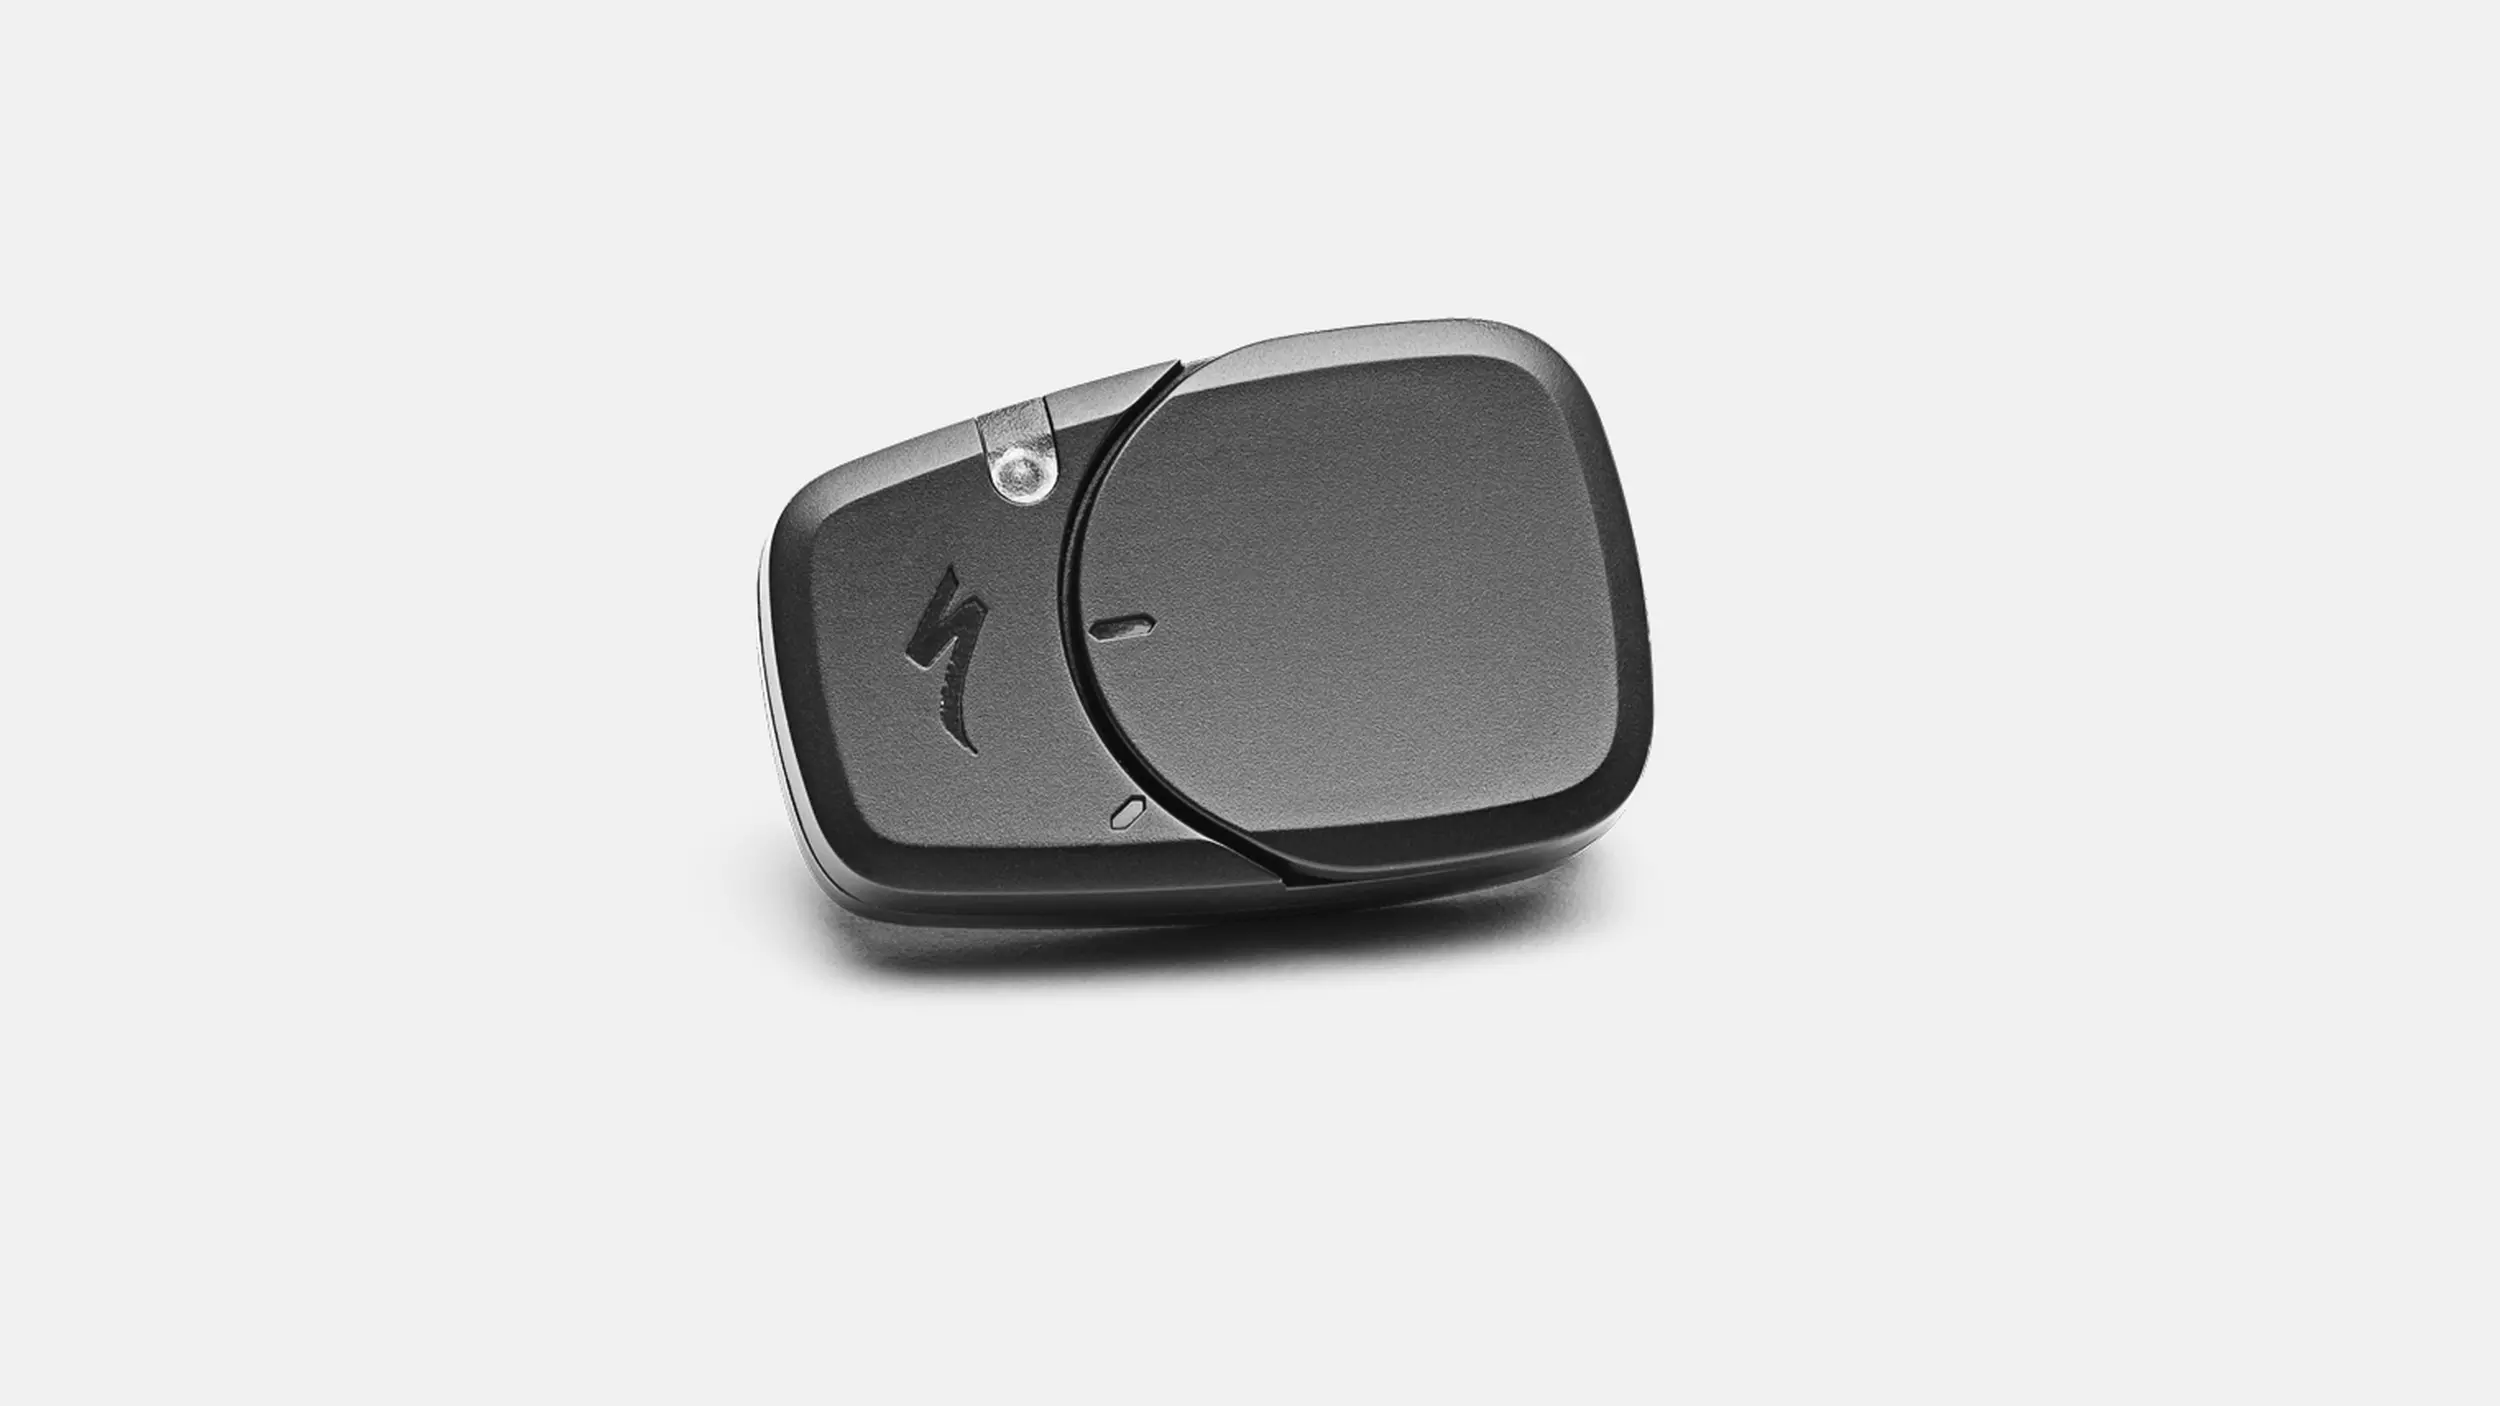
\includegraphics[width=7cm]{Graphics/angi.png}
\centering
\caption{Urządzenie ANGI, stworzone przez firmę Specialized \cite{ANGI}}.
\centering
\label{img:angi_img}
\end{figure}

%---------------------------------------------------------------------------















\chapter{Prototyp urządzenia pomiarowego}
\label{cha:prototyp}


\section{TODO}
TODO Some text
\begin{itemize}
    \item A
    \item B
    \item C
\end{itemize}
%TODO: Podmienić zdjęcie urządzenia testowego

\chapter{TODO}
\section{TODO}
\chapter{TODO}
\section{TODO}
\section{Kierunki rozwoju}

\chapter{Podsumowanie}




% itd.
% \appendix
% \include{dodatekA}
% \include{dodatekB}
% itd.

\printbibliography

\end{document}